%TCIDATA{LaTeXparent=0,0,relatorio.tex}

\chapter{Diagramas El�tricos e Tabelas de Sinais}

\begin{table}[h]
\centering
\begin{tabu}{l|l|[2pt]l|l}
M�dulo                                & Pino                     & M�dulo               & Pino    \\ \tabucline[2pt]{-}
AC Power Cord                         & L                       & SWITCH               & 1      \\ \hline
AC Power Cord                         & N                       & SWITCH               & 2      \\ \hline
\multirow{2}{*}{AC Power Cord}        & \multirow{2}{*}{G}      & 24Vdc Power Supply 1 & G      \\ \cline{3-4} 
                                      &                         & 24Vdc Power Supply 2 & G      \\ \hline
SWITCH                                & 4                       & 6A fuse              & IN     \\ \hline
\multirow{2}{*}{SWITCH}               & \multirow{2}{*}{3}      & 24Vdc Power Supply 1 & N      \\ \cline{3-4} 
                                      &                         & 24Vdc Power Supply 2 & N      \\ \hline
\multirow{2}{*}{6A fuse}              & \multirow{2}{*}{OUT}    & 24Vdc Power Supply 1 & L      \\ \cline{3-4} 
                                      &                         & 24Vdc Power Supply 2 & L      \\ \hline
\multirow{2}{*}{24Vdc Power Supply 1} & \multirow{2}{*}{+24Vdc} & PLC Touch Panel      & 24 Vdc \\ \cline{3-4} 
                                      &                         & C1                   & 5      \\ \hline
24Vdc Power Supply 2                  & +24Vdc                  & Relay                & 87     \\ \hline
\multirow{4}{*}{24Vdc Power Supply 1} & \multirow{4}{*}{GND}    & 24Vdc Power Supply 2 & GND    \\ \cline{3-4} 
                                      &                         & C1                   & 6      \\ \cline{3-4} 
                                      &                         & Relay                & 85     \\ \cline{3-4} 
                                      &                         & Sabertooth2x60       & B-     \\ \hline
C1                                    & 4                       & C1                   & 9      \\ \hline
Relay                                 & 86                      & C6                   & 10     \\ \hline
C5                                    & 8                       & C6                   & 11     \\ \hline
Relay                                 & 30                      & Sabertooth2x60       & B+     \\ \hline
Sabertooth2x60                        & M2B                     & M\_WHITE             & -      \\ \hline
Sabertooth2x60                        & M2A                     & M\_WHITE             & +      \\ \hline
Sabertooth2x60                        & M1B                     & M\_RED               & -      \\ \hline
Sabertooth2x60                        & M1A                     & M\_RED               & +      \\ \hline
\multirow{2}{*}{C4}                   & \multirow{2}{*}{12}     & 10K R2               & +      \\ \cline{3-4} 
                                      &                         & Sabertooth2x60       & S1     \\ \hline
\multirow{2}{*}{C4}                   & \multirow{2}{*}{9}      & 10K R1               & +      \\ \cline{3-4} 
                                      &                         & Sabertooth2x60       & S2     \\ \hline
\multirow{4}{*}{C4}                   & \multirow{4}{*}{7}      & C4                   & 10     \\ \cline{3-4} 
                                      &                         & 10K R2               & -      \\ \cline{3-4} 
                                      &                         & 10K R1               & -      \\ \cline{3-4} 
                                      &                         & Sabertooth2x60       & 0V     \\ 
\end{tabu}
\caption{Tabela de sinais para o diagrama el�trico principal.}
\label{tab:SigMain}
\end{table}

\begin{table}[h]
\centering
\begin{tabu}{l|l|[2pt]l|l}
M�dulo                                & Pino                     & M�dulo               & Pino    \\ \tabucline[2pt]{-}
\multirow{2}{*}{LIMIT SWITCHER Red\_Ret} & \multirow{2}{*}{GND}  & LIMIT SWITCHER Red\_Ext & GND            \\ \cline{3-4} 
                                         &                       & C5                      & GND            \\ \hline
\multirow{3}{*}{LIMIT SWITCHER Red\_Ret} & \multirow{3}{*}{Vcc}  & LIMIT SWITCHER Red\_Ext & Vcc            \\ \cline{3-4} 
                                         &                       & 2.7K R3                 & +              \\ \cline{3-4} 
                                         &                       & 2.7K R4                 & +              \\ \hline
\multirow{2}{*}{LIMIT SWITCHER Red\_Ret} & \multirow{2}{*}{OUT}  & 2.7K R3                 & -              \\ \cline{3-4} 
                                         &                       & C5                      & DI 1           \\ \hline
\multirow{2}{*}{LIMIT SWITCHER Red\_Ext} & \multirow{2}{*}{OUT}  & 2.7K R4                 & -              \\ \cline{3-4} 
                                         &                       & C5                      & DI 2           \\ \hline
Red encoder                              & Vcc                   & C8                      & Encoder 24 V + \\ \hline
Red encoder                              & GND                   & C8                      & GND            \\ \hline
Red encoder                              & A                     & C8                      & A              \\ \hline
Red encoder                              & B                     & C8                      & B              \\ \hline
\multirow{2}{*}{LIMIT SWITCHER Whi\_Ret} & \multirow{2}{*}{GND}  & LIMIT SWITCHER Whi\_Ext & GND            \\ \cline{3-4} 
                                         &                       & C7                      & GND            \\ \hline
\multirow{3}{*}{LIMIT SWITCHER Whi\_Ret} & \multirow{3}{*}{Vcc}  & LIMIT SWITCHER Whi\_Ext & Vcc            \\ \cline{3-4} 
                                         &                       & 2.7K R7                 & +              \\ \cline{3-4} 
                                         &                       & 2.7K R8                 & +              \\ \hline
\multirow{2}{*}{LIMIT SWITCHER Whi\_Ret} & \multirow{2}{*}{OUT}  & 2.7K R7                 & -              \\ \cline{3-4} 
                                         &                       & C7                      & DI 1           \\ \hline
\multirow{2}{*}{LIMIT SWITCHER Whi\_Ext} & \multirow{2}{*}{OUT}  & 2.7K R8                 & -              \\ \cline{3-4} 
                                         &                       & C7                      & DI 2           \\ \hline
White encoder                              & Vcc                   & C9                      & Encoder 24 V + \\ \hline
White encoder                              & GND                   & C9                      & GND            \\ \hline
White encoder                              & A                     & C9                      & A              \\ \hline
White encoder                              & B                     & C9                      & B              \\ \hline
Pressure Sensor Red                      & V+                    & C1                      & +24 V I/O (4)  \\ \hline
\multirow{2}{*}{Pressure Sensor Red}     & \multirow{2}{*}{Vout} & C3                      & AI + 1 U       \\ \cline{3-4} 
                                         &                       & 249 R5                  & +              \\ \hline
Pressure Sensor White                    & V+                    & C1                      & +24 V I/O (5)  \\ \hline
\multirow{2}{*}{Pressure Sensor White}   & \multirow{2}{*}{Vout} & C3                      & AI + 3 U       \\ \cline{3-4} 
                                         &                       & 249 R6                  & +              \\ \hline
\multirow{3}{*}{249 R5}                  & \multirow{3}{*}{-}    & C3                      & AI - 1 U       \\ \cline{3-4} 
                                         &                       & C3                      & AI - 3 U       \\ \cline{3-4} 
                                         &                       & 249 R6                  & -              \\ \hline
\end{tabu}
\caption{Tabela de sinais para o diagrama el�trico de sensores.}
\label{tab:SigSens}
\end{table}
%\newpage
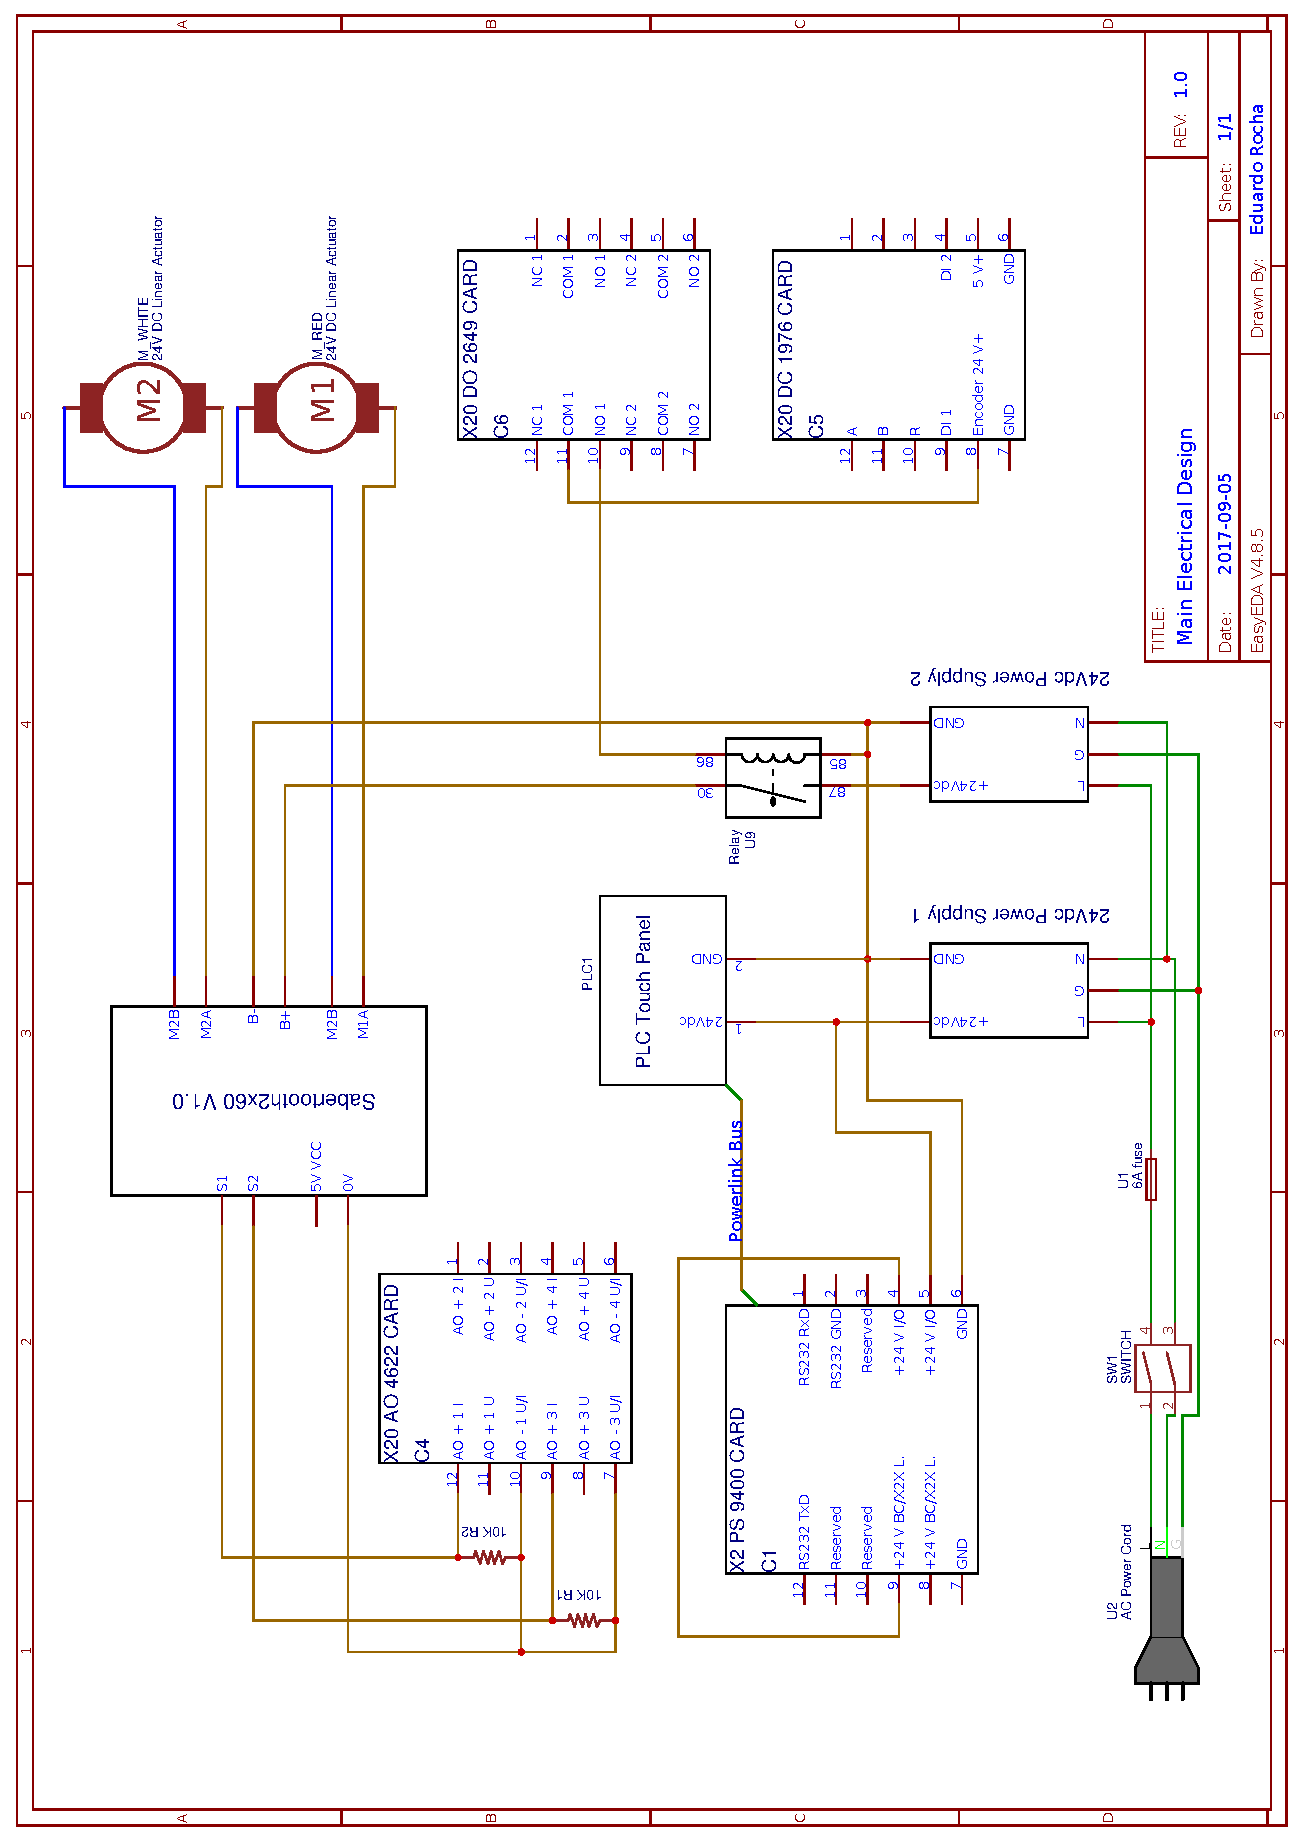
\includepdf[pages={1,2}]{Electrical.pdf}






\refstepcounter{noAnexo}
\chapter{Desenhos T�cnicos das Pe�as Usinadas}

\begin{figure}[h]
\centering
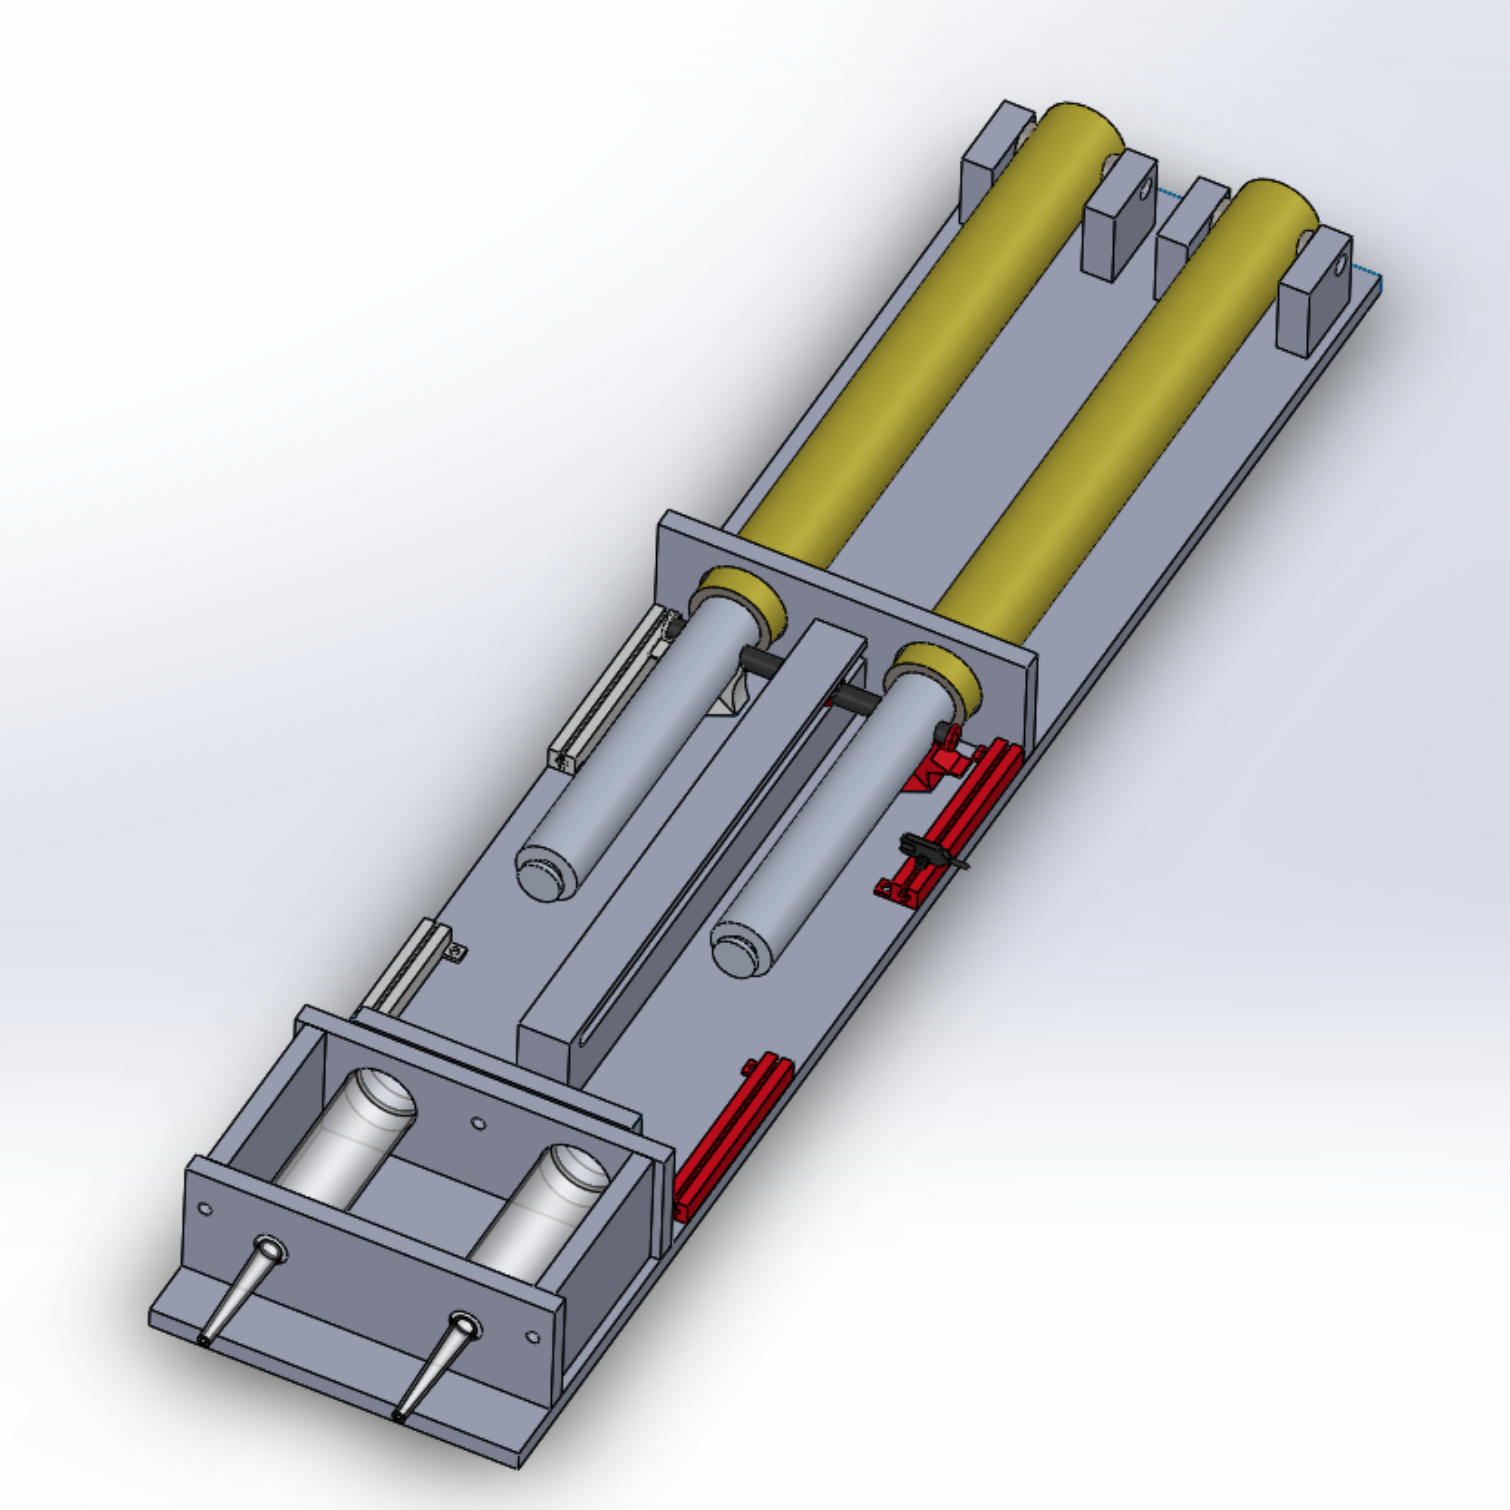
\includegraphics[width = \textwidth]{figs/desenho3D}
\caption{Desenho 3D da bomba injetora feito no SolidWorks.}
\end{figure}

\includepdf[pages = {2,3,4,5,6}]{Drawings.pdf}

\refstepcounter{noAnexo}
\chapter{P�ginas da Interface de Usu�rio}

\begin{figure}[h]
\centering
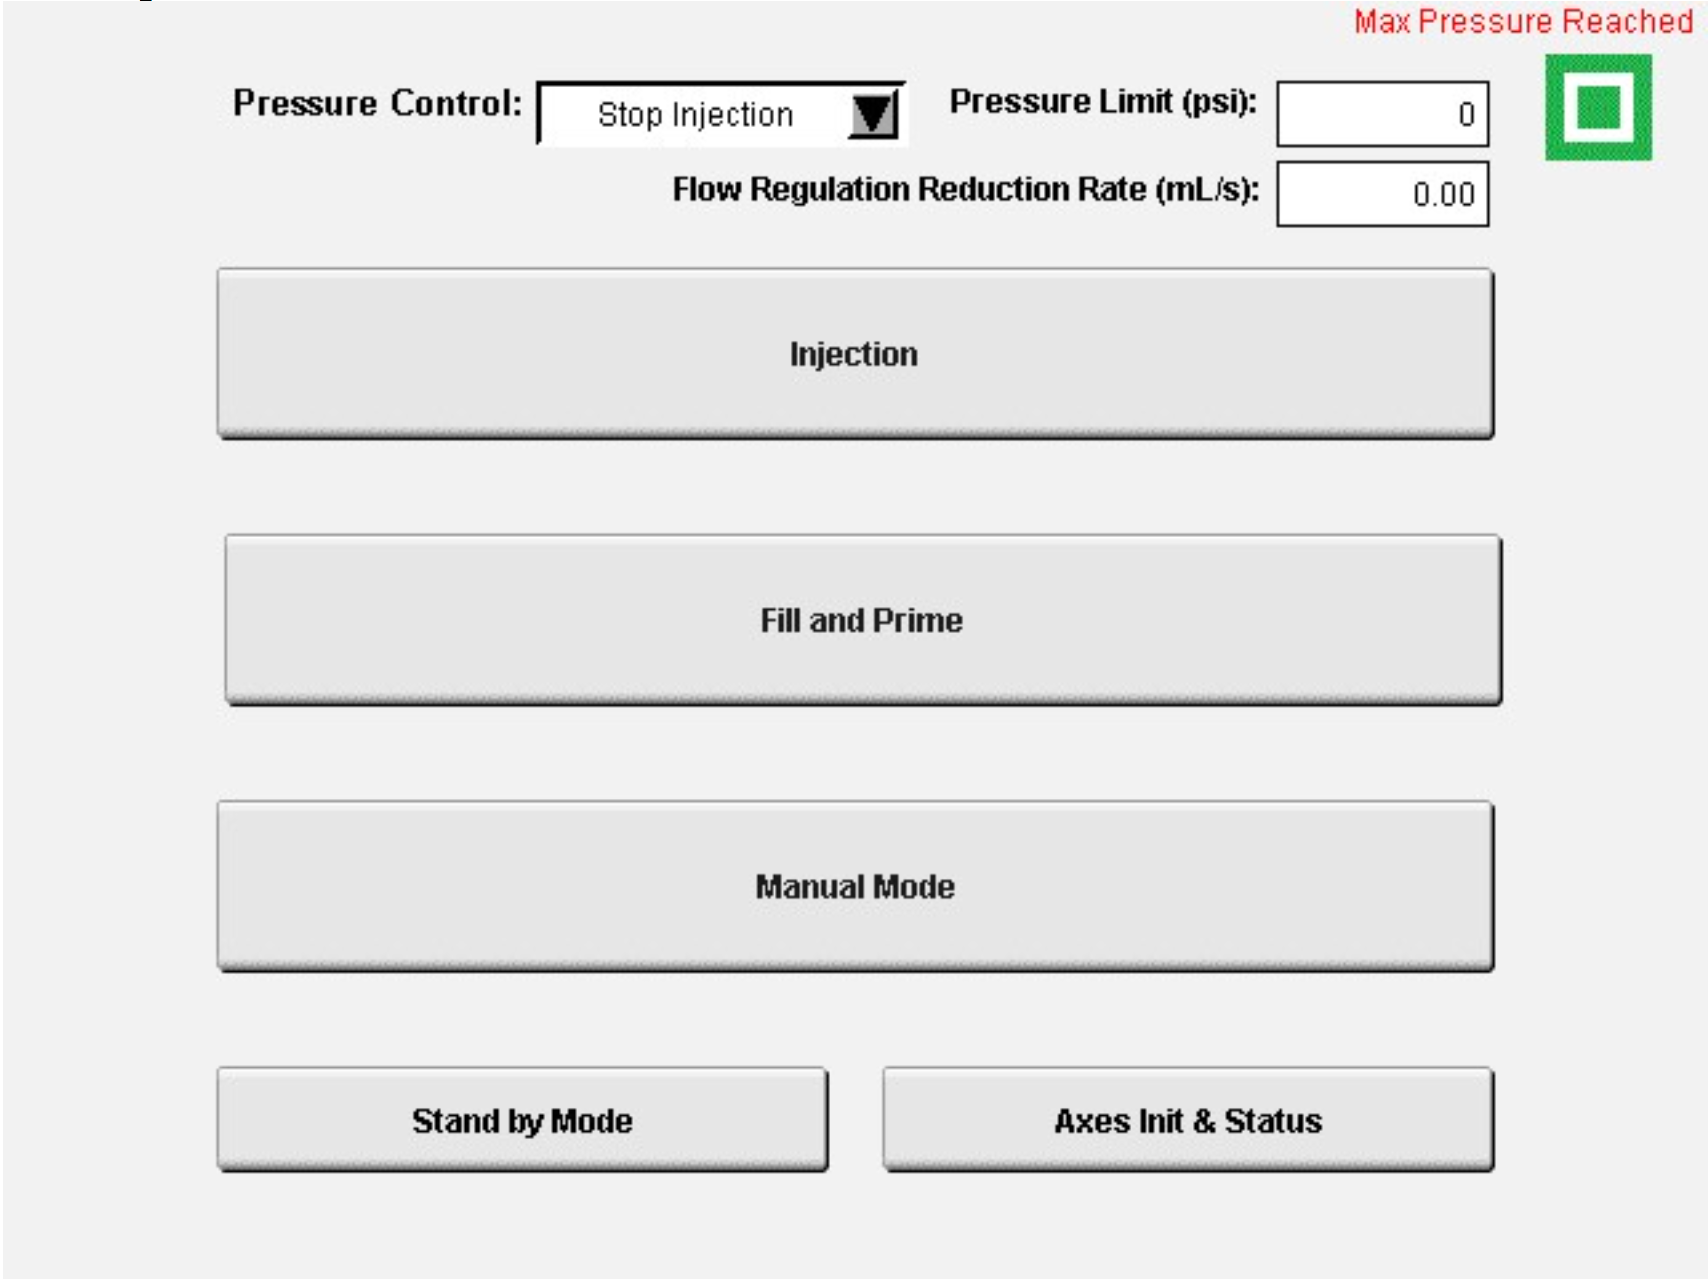
\includegraphics[width = 0.8\textwidth]{figs/InitPage}
\caption{P�gina inicial da Interface de Usu�rio.}
\end{figure}
\begin{figure}[h]
\centering
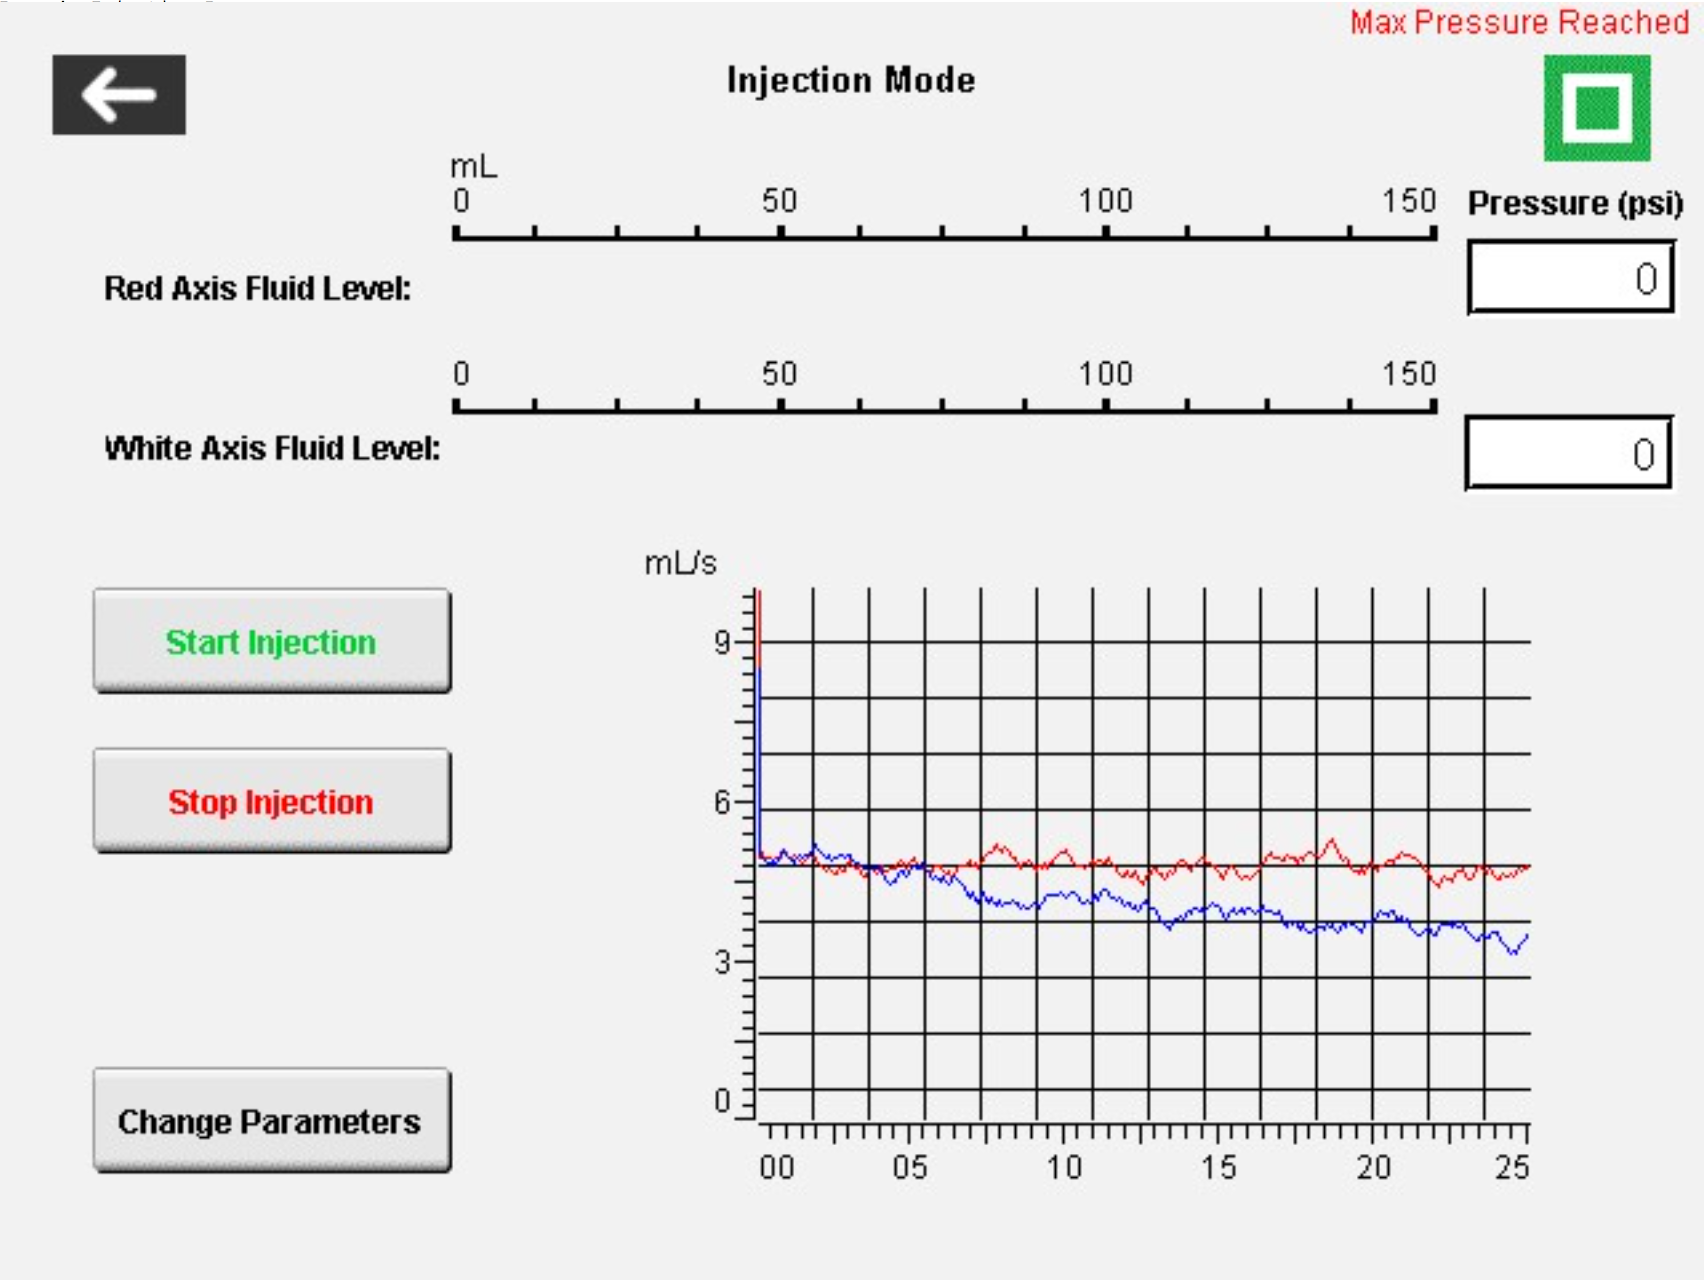
\includegraphics[width = 0.8\textwidth]{figs/InjePage}
\caption{P�gina de inje��o da Interface de Usu�rio.}
\end{figure}
\begin{figure}[h]
\centering
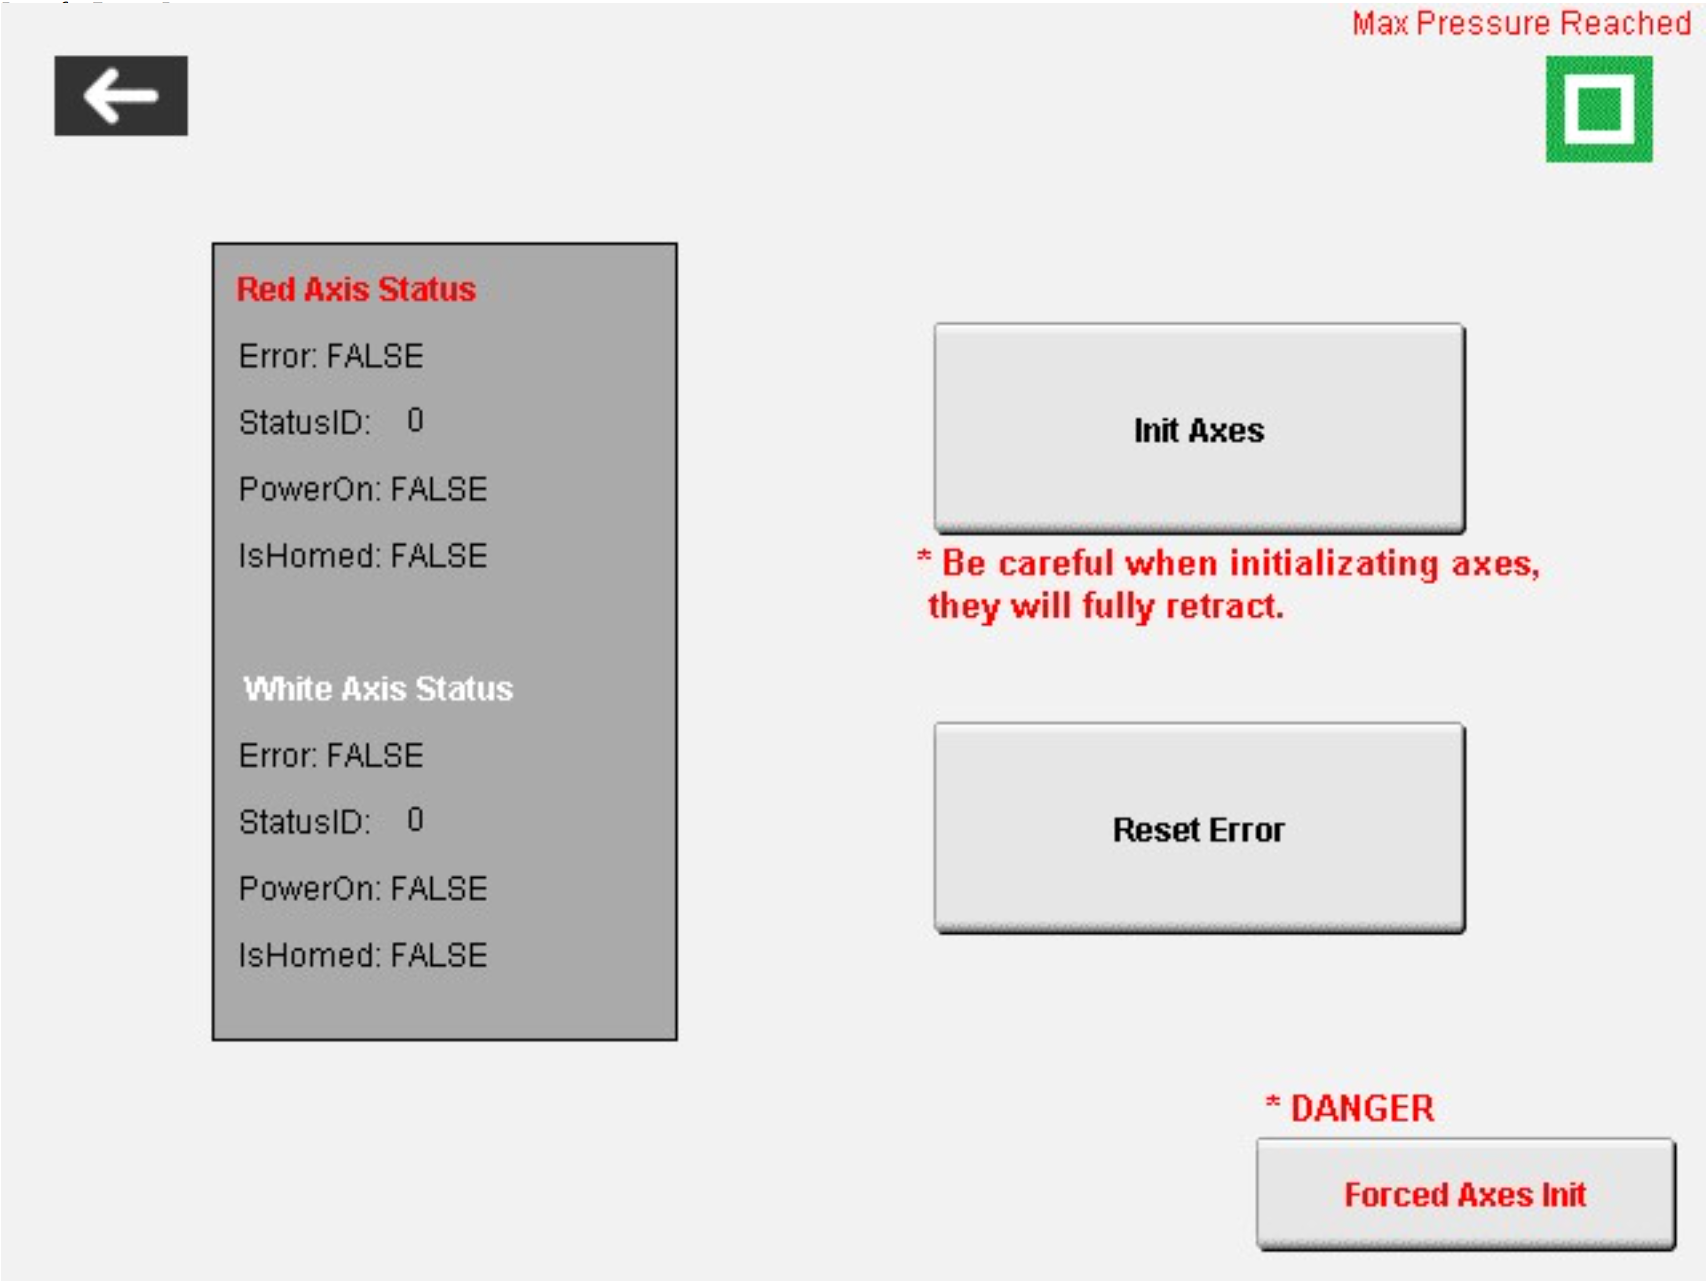
\includegraphics[width = 0.8\textwidth]{figs/ErrorPage}
\caption{P�gina de erros da Interface de Usu�rio.}
\end{figure}
\begin{figure}[h]
\centering
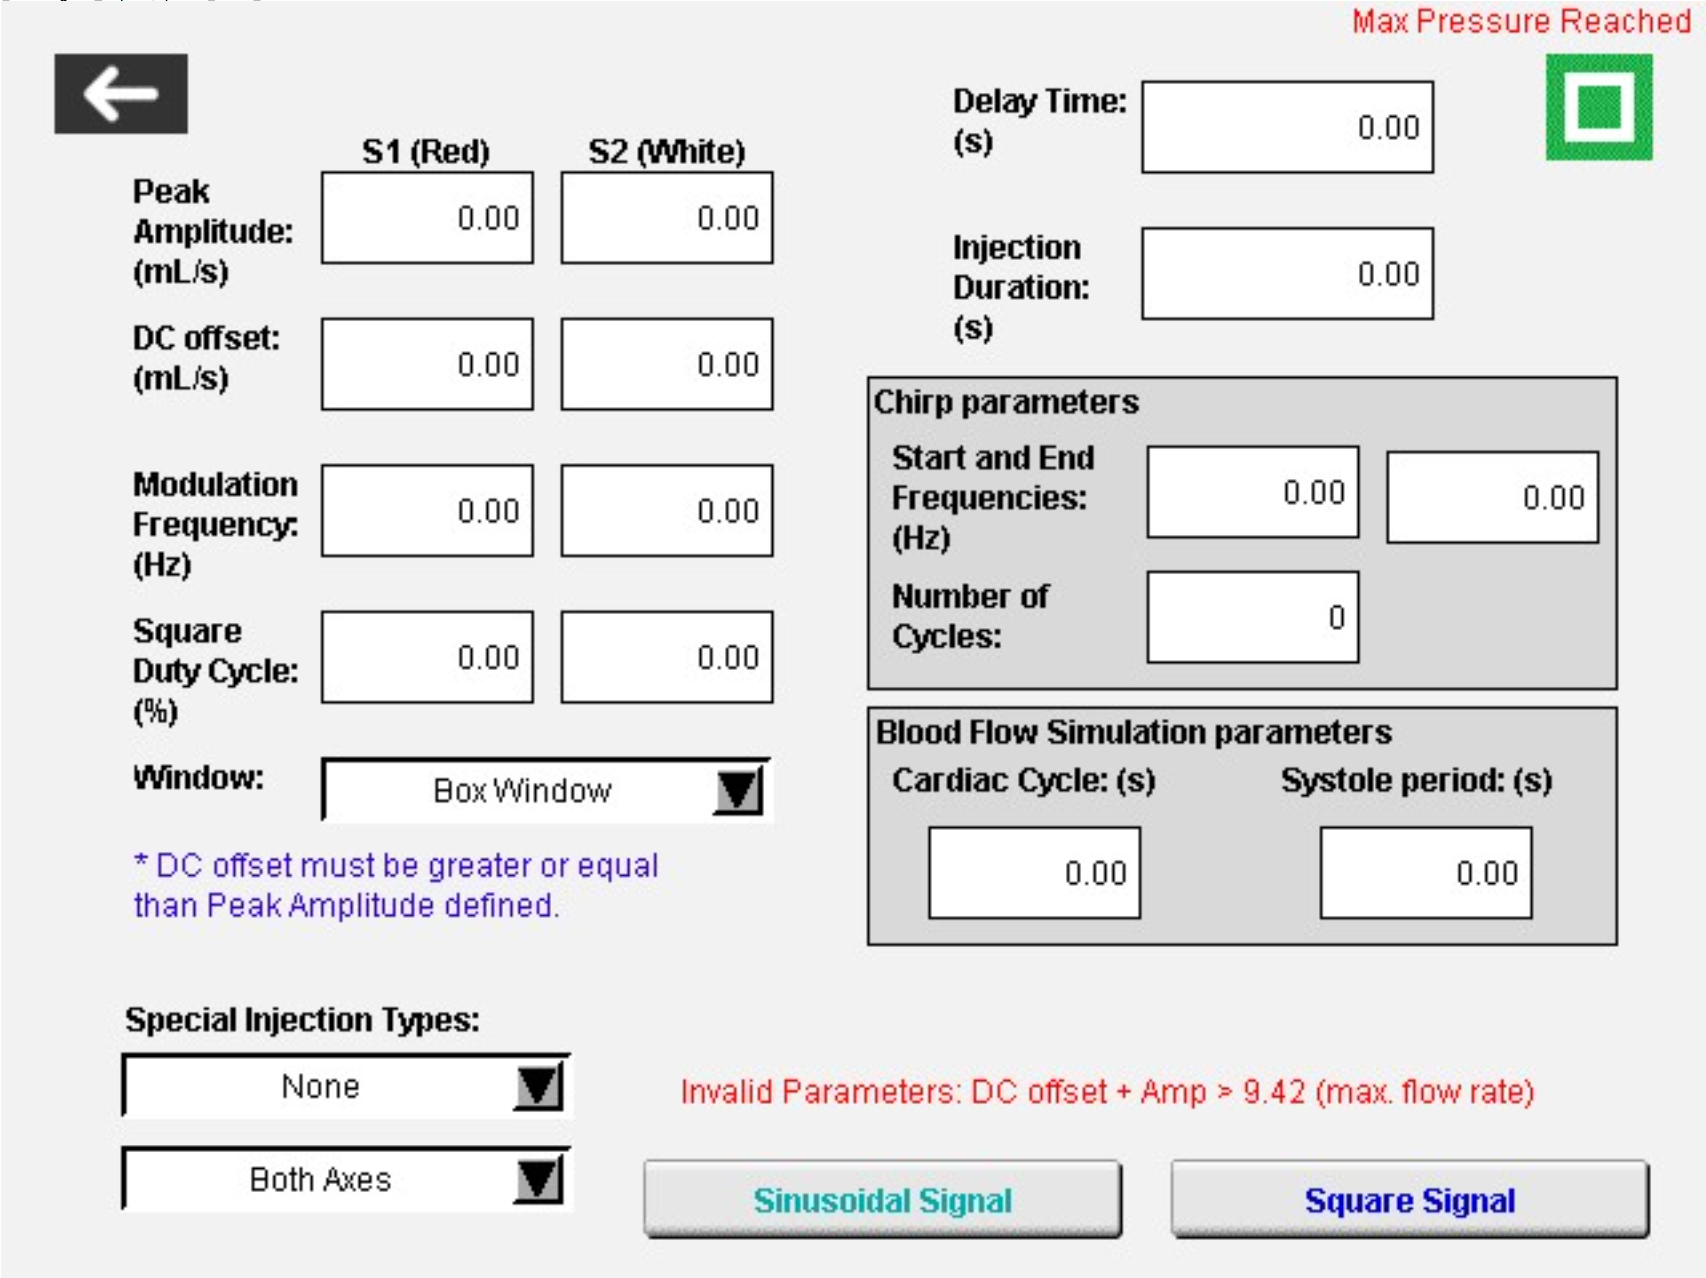
\includegraphics[width = 0.8\textwidth]{figs/ParPage}
\caption{P�gina de par�metros de inje��o da Interface de Usu�rio.}
\end{figure}
\begin{figure}[h]
\centering
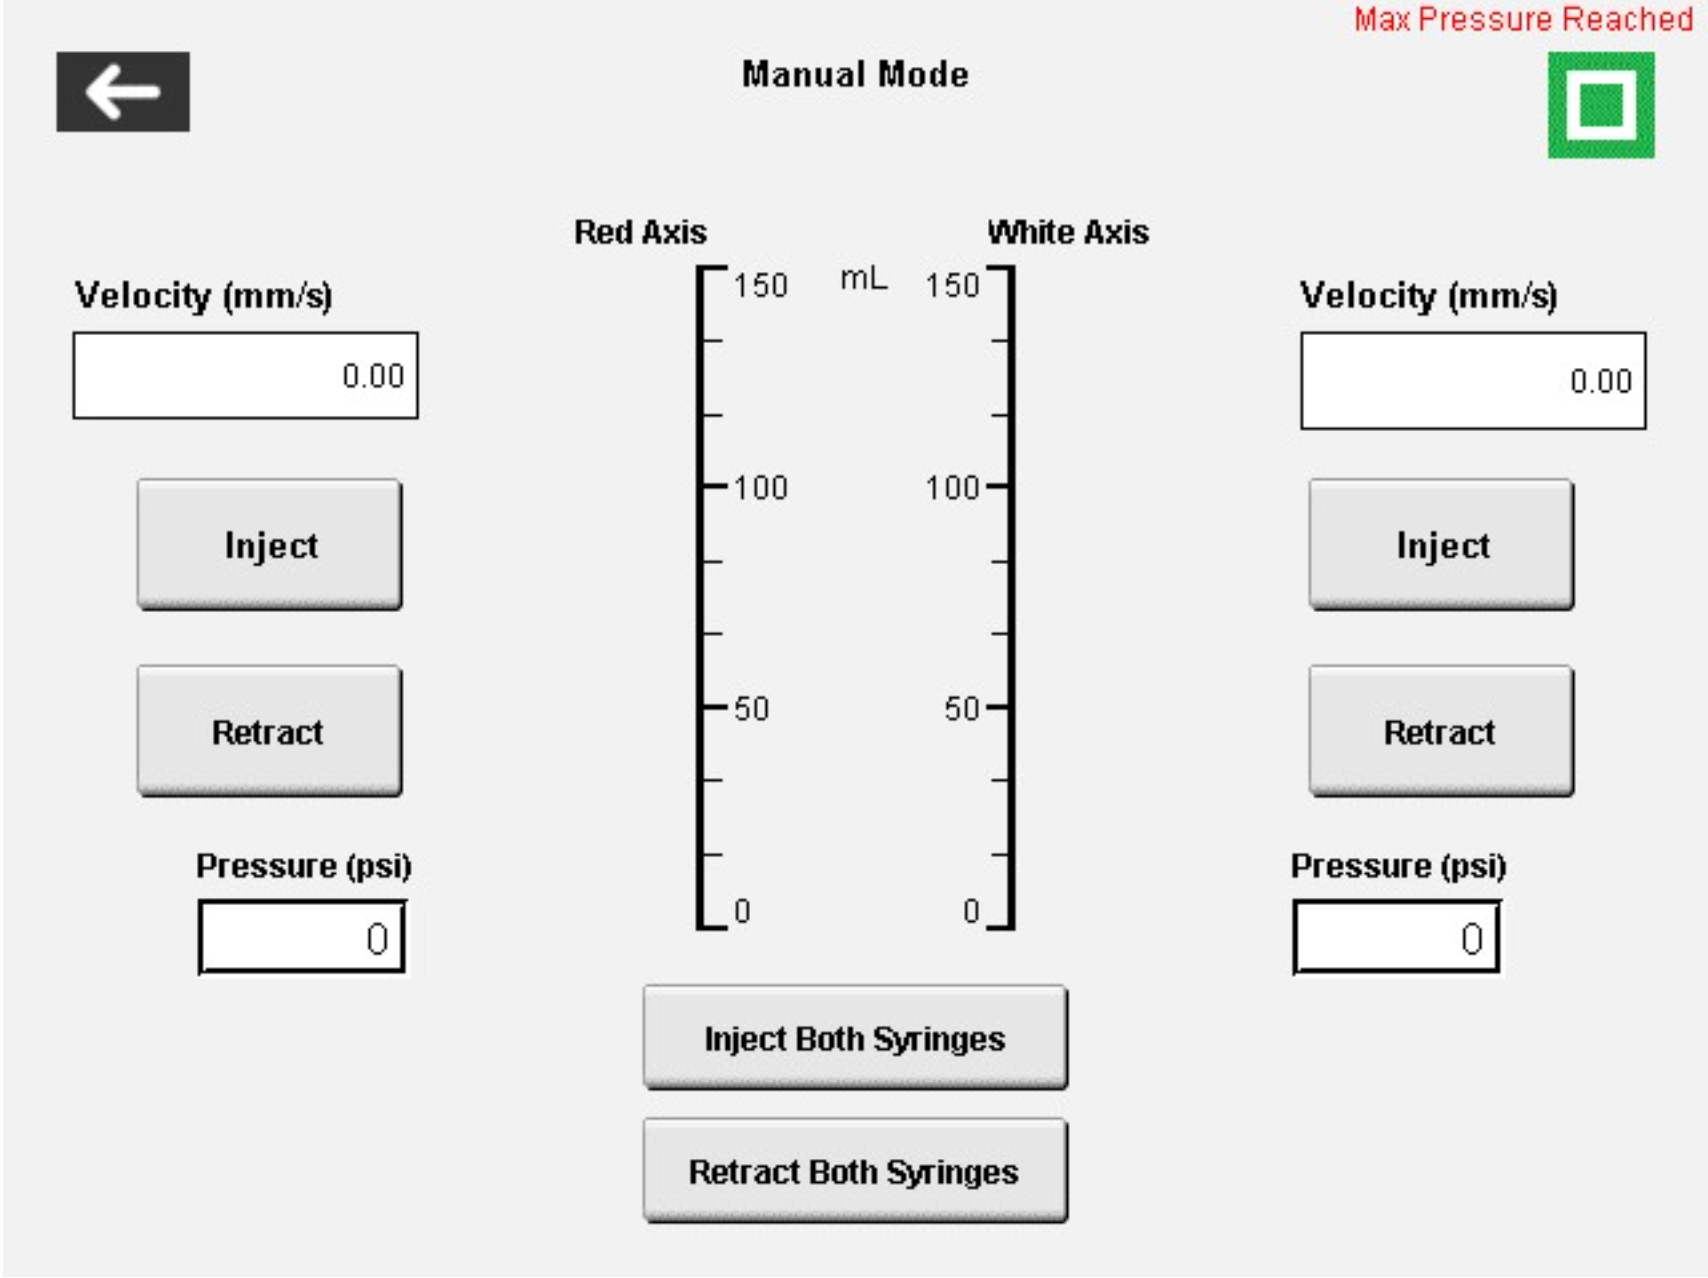
\includegraphics[width = 0.8\textwidth]{figs/ManualPage}
\caption{P�gina de opera��o manual da Interface de Usu�rio.}
\end{figure}
\begin{figure}[h]
\centering
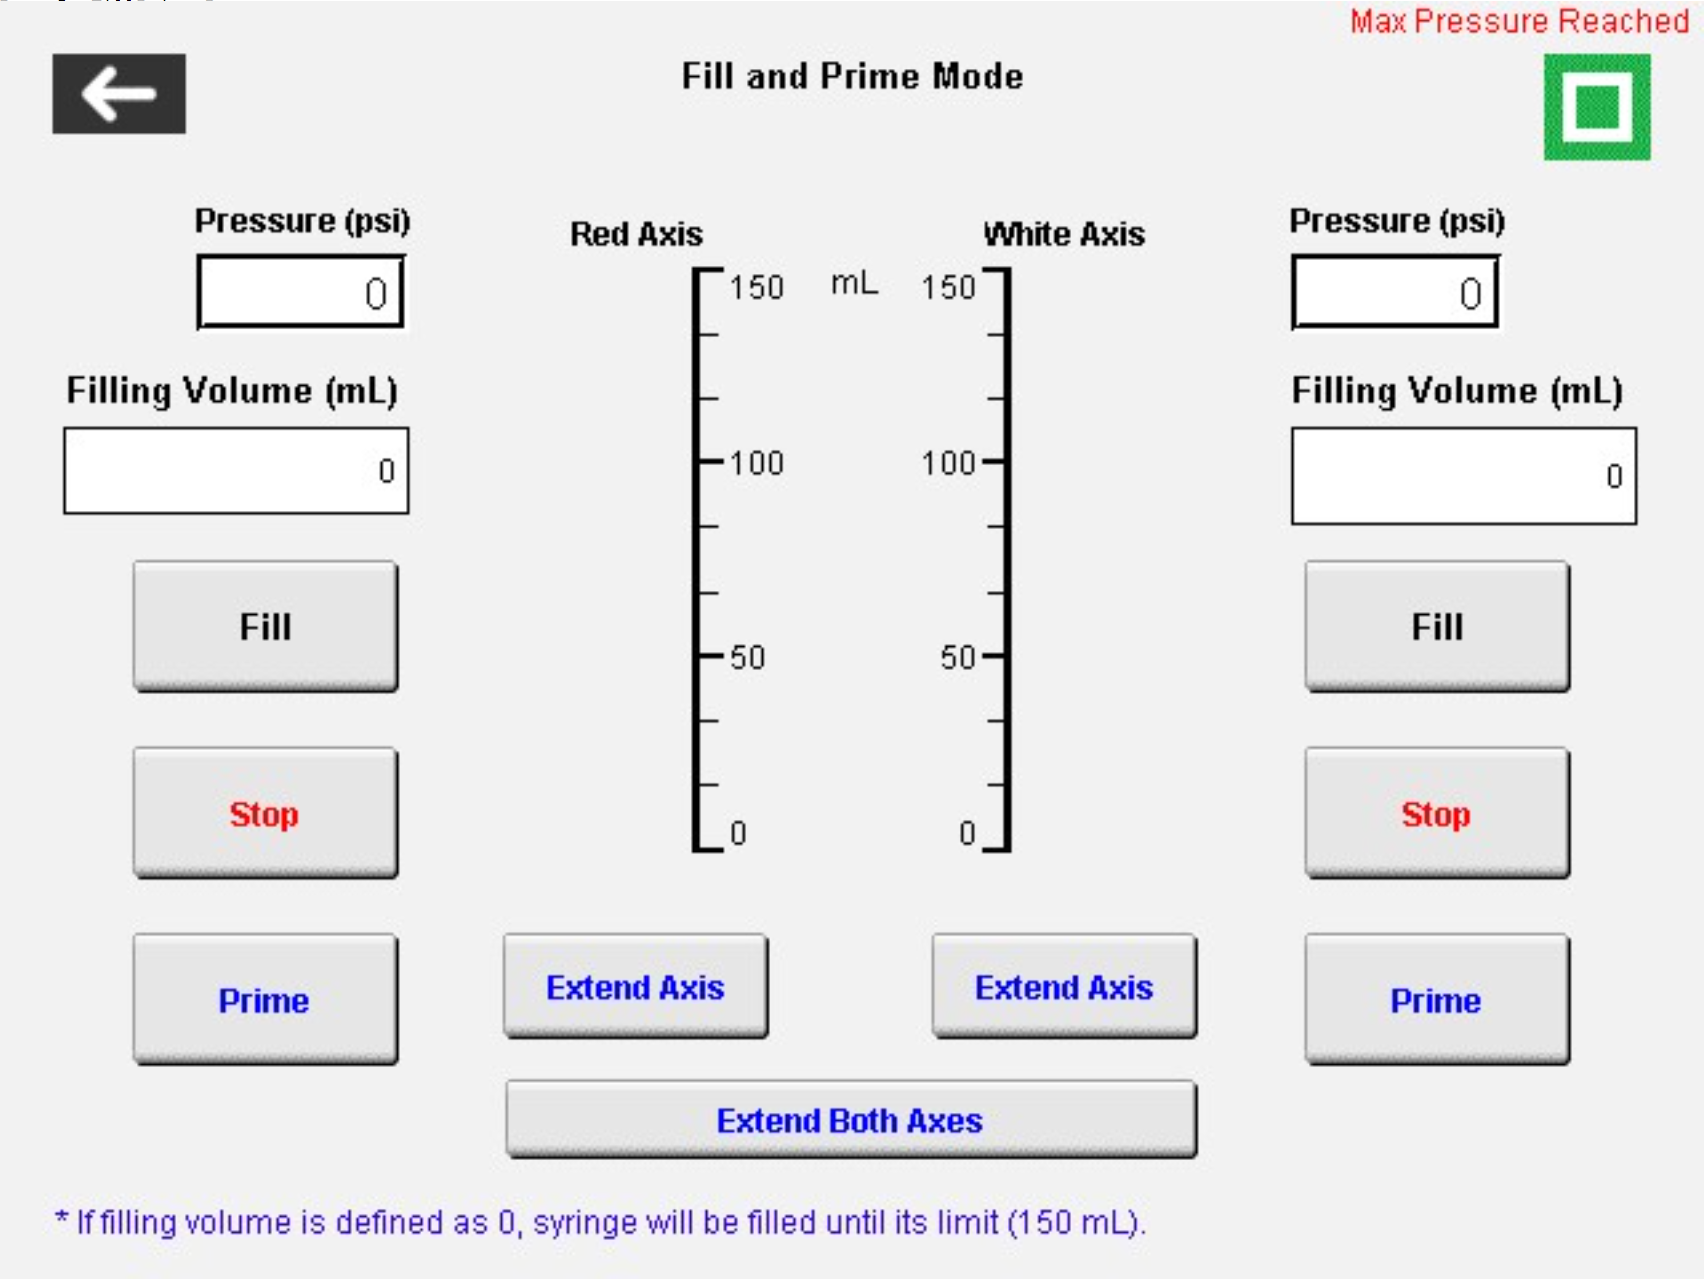
\includegraphics[width = 0.8\textwidth]{figs/FillPage}
\caption{P�gina de enchimento da Interface de Usu�rio.}
\end{figure}
